%% This is an example first chapter.  You should put chapter/appendix that you
%% write into a separate file, and add a line \include{yourfilename} to
%% main.tex, where `yourfilename.tex' is the name of the chapter/appendix file.
%% You can process specific files by typing their names in at the 
%% \files=
%% prompt when you run the file main.tex through LaTeX.
\chapter{Implementation}

\section{Cyclic Reduction}


Cyclic reduction (CR) is an algorithm introduced by G. H. Golub and R. W. Hoekney [1] in the mid 1960s for solving tridiagonal linear systems related to the finite difference discretization of the Poisson equation over a rectangle. 
The basic idea of the CR algorithm , also called odd-even reduction, is to eliminate half the unknowns, regroup the equations in even and odd numbered and again eliminate half the unknowns.


\subsection{The algorithm}

CR method only applies to matrices that can be represented as a (block) Toeplitz matrix; such problems often arise in implicit solutions for partial differential equations on a lattice. For example fast solvers for Poisson's equation express the problem as solving a tridiagonal matrix, discretising the solution on a regular grid. From 1D Poisson’s equation arises a tridiagonal matrix system while from 2D Poisson’s equation arises a block tridiagonal system.
In general large tridiagonal systems of linear equations appear in many numerical analysis applications. A tri-diagonal matrix is a matrix with values only in the sub-, main- and super-diagonal.

For example, the tridiagonal system:

$a_i*x_{i-1} + b_i*x_i+c_i*x_{i+1} = F_{i}$  , \hspace*{2cm} $ i=1:1:n$

Assume that $n= 2^p - 1$. 
The algorithm proceeds in two steps: a forward reduction and a backward substitution. Each phase consists of ($\log_2n – 1$) steps, where n is the system size. The first step in cyclic reduction is to combine linearly the equations in order to eliminate the odd numbered unknowns ($x_1$, $x_3$ … $x_n$). Next the unknowns are re-ordered and the process is continued until the system consists from one equation with one unknown. To do this the algorithm is based to triplets. In the above example in order to eliminate $x_1$ and $x_3$,the first three equations of the system are chosen and multiplied by the parameters $\alpha_2$, $\beta_2$, $\gamma_2$. \\
\\
$b_1*x_1+c_1*x_2= F_1$                        \hspace*{5cm} $*(\alpha_2)$	\\
$a_2*x_1+ b_2*x_2+c_2*x_3= F_2$               \hspace*{3,3cm} $* (\beta_2)$  \\
\hspace*{2cm}$a_3*x_2+ b_3*x_3+c_3*x_4= F_3$  \hspace*{1,3cm} $*(\gamma_2)$     \\ \\
Subsequently the equations are summed and we have the resulted equation. Similarly this elimination process proceeds for the next three equations, until we have only one equation.
Using the back substitution the unknown x can be calculated from the last one equation and  all the others $x_i$ can be found  from the previous steps .The described steps can be illustrated in Figure 4-1.\\


\begin{figure}[h]
   \centering
       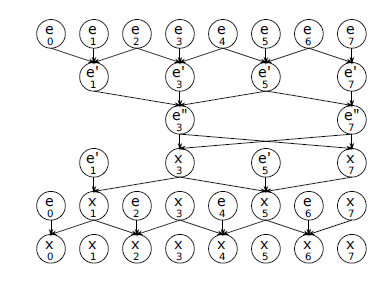
\includegraphics[width=0.5\textwidth]{cr}
   \caption{cr method}
   \label{fig:gpuarch}
\end{figure}
As it is said a tridiagonal matrix has basically 3 diagonals, (super, main, sub). In order to take advantage of this, we can consider that the matrix consists from three vectors and store only these three vectors plus one vector for the right hand side of the system.
If we consider that vector a is the sub-diagonal, vector c is the supper diagonal, vector b is the main diagonal and vector F is the right hand side, pseudo code for the forward elimination is given below: \\
$a_i*x_{i-1} + b_i*x_i+c_i*x_{i+1} = F_{i}  ,   i=1:1:n$
\begin{algorithm}[H]
\begin{algorithmic}[1]
\Function{Forward Reduction}{}
\State{for$(i=0;  i<\log_2(size+1)-1; i++)$\{}
	 \State{\hspace*{1cm}for$(j=2^{i+1}-1; j<size; j=j+2^{i+1})$\{}
	    \State{\hspace*{2cm}$offset = pow(2,i);$}
        \State{\hspace*{2cm}$index_1=j-offset;$}        
        \State{\hspace*{2cm}$k_1 = a[j]/b[index_1];$}
        \State{\hspace*{2cm}$k_2 = c[j]/b[j];$}
        \State{\hspace*{2cm}$b[j] = b[j] - c[j-offset] * k_1 - a[j+offset] * k_2;$}
        \State{\hspace*{2cm}$F[j] = F[j] - F[j-offset] * k_1 - F[j+offset] * k_2;$}
        \State{\hspace*{2cm}$a[j] = -a[j-offset] * k_1;$}
        \State{\hspace*{2cm}$c[j] = -c[j+offset] * k_2;$}
        \State{\hspace*{2cm}\}}
      \State{\}} 
\EndFunction
\end{algorithmic}
\caption{Cyclic Reduction - Forward}
\label{alg:forward_cr}
\end{algorithm}
After the forward elimination the resulting system is one equation with one unknown. Hereafter, it is trivial to deduce the remaining unknowns. Formally the resulting solution can be calculated by following pseudo code:
\begin{algorithm}[H]
\begin{algorithmic}[1]
\Function{Backward Substitution (first step)}{}
\State{$int index = (size-1)/2;$} 
\State{$x[index] = F[index]/b[index];$} 
\EndFunction
\end{algorithmic}
\caption{Cyclic Reduction - Backward-First step}
\label{alg:Backwardfirst_cr}
\end{algorithm}


\begin{algorithm}[H]
\begin{algorithmic}[1]
\Function{Backward Substitution}{}
\State{for$(i=\log_2(size+1)-2;i>=0;i--)$\{ }
	 \State{\hspace*{1cm}for$(j=2^{i+1}-1;j<size;j=j+2^{i+1})$\{ }
	    \State{\hspace*{2cm}$offset = 2^i;$}
        \State{\hspace*{2cm}$index_1 = j-offset;$}        
        \State{\hspace*{2cm}$index_2 = j+offset;$}        
        \State{\hspace*{2cm}$if(j!=index_1)$}
       		\State{\hspace*{3cm}$ x[index_1] = (F[index_1] - a[index_1]*x[index_1-offset] - c[index_1]*x[index_1+offset])/b[index_1];$}
        \State{\hspace*{2cm}$if(j!=index_2)$}
        	\State{\hspace*{3cm}$x[index_2] = (F[index_2] - a[index_2]*x[index_2-offset] - c[index_2]*x[index_2+offset])/b[index_2];$}    
        	\State{\hspace*{2cm}\}}
        	\State{\}} 
\EndFunction
\end{algorithmic}
\caption{Cyclic Reduction - Backward}
\label{alg:Backward_cr}
\end{algorithm}


\subsection{Implementation Issues}


The first goal was to run all the steps of CR on GPU. As we can understand from the pseudo code there are dependences between data during the outer for loop for both forward and backward step. 
Subsequently, the first Kernel for forward elimination called in this way
\begin{algorithmic}
\For {$i=\log_2(size+1)-2;i>=0;i--$}\\
 \hspace*{1cm}<Kernel forward>
\EndFor
\end{algorithmic}


keeping as parameter the necessary step size. Step size, essentially, settles on the termination condition for the kernel. The dimension of the grid and the block are determined through the following function.

\begin{algorithm}[H]
\begin{algorithmic}[1]
\Function{Calculate Block Dimension}{size,block,grid}
\State{if$(size<4)$\{$block->x=1;block->y=1;$\}}
\State{else if$(size<16)$\{$block->x=2;block->y=2;$\}}
\State{else if$(size<64)$\{$block->x=4;block->y=4;$\}}
\State{else if$(size<256)$\{$block->x=8;block->y=8;$\}}	
\State{else \{$block->x=16;block->y=16;$\}}
\EndFunction
\end{algorithmic}
\caption{Block Dimension}
\label{alg:calc_dim}
\end{algorithm}
In other words, the geometry changes while the size of the system is growing. 
Likeness for the backward substitution step, it is determined the stepsize and the block dimension.
Before the kernel’s launches, all vectors (three diagonals and one for the right side hand) are transferred from host to device using continuous CudaMemcpy(). It is also necessary to initialize to zero the resulting vector x using CudaMemSet(), because it takes parts to computations. Finally the result vector is transferred from the device to host.

\section{Block Cyclic Reduction}

The basic idea of the cyclic reduction method can be extended to block tridiagonal systems. The idea of the block cyclic reduction (BCR) was first introduced by Gene Golub to deal with the scalar tridiagonal systems that arise from the finite element discretization of the Poisson equation in 2D. As in cyclic reduction, block cyclic reduction is a two phase algorithm. It consists of forward reduction and backward substitution. During each step of the reduction stage, are eliminated approximately half the unknowns in the system. After $O(\log_2 n)$ reductions a $1x1$ block system is left. After solving this system, the previously eliminated unknowns are computed by back substitution. While this formulation is numerically unstable, O. Buneman suggested a stable variation.  In this thesis, we consider the case of block cyclic reduction, where the scalar elements of traditional cyclic reduction are replaced with matrix tridiagonal and diagonal blocks.

\subsection{The algorithm}

The implemented algorithm solves systems of the following form:
 $A*U = F$\\  
where the \emph{A} is a block tridiagonal matrix: 
\[ \left( \begin{array}{ccccc}
B  & T &     &   &\\
T  & B &  T  &    &\\
   & T &  B  & T  &\\
   &   & ...    &    &  \\     
   &   &     & ...  &  \\
   &   &  T  & B & T \\    
   &   &     & B & T\\	
    \end{array} \right)\] 
where B is a tridiagonal matrix. For example a typical tridiagonal matrix arising from 
Poisson discretization is : \\
the \emph{B Matrix}
\[ \left( \begin{array}{ccc}
-4 & 1 &  \\
1  & -4 & -1 \\
   & -1 & -4 \end{array} \right)\] 
and T is either the \emph{Identical Matrix}
\[ \left( \begin{array}{ccc}
1 & 0 & 0 \\
0 & 1 & 0 \\
0 & 0 & 1 \end{array} \right)\] or The \emph{-Identical Matrix}
\[ \left( \begin{array}{ccc}
-1 & 0 & 0 \\
0 & -1 & 0 \\
0 & 0 & -1 \end{array} \right)\] 
\\

The concept of block cyclic reduction is to iteratively eliminate half of the unknowns until there is an only single
block system which can be solved directly. 
So we have for such as : $1 < j < 2^jq -1$\\
$TU_{2*j-2} + BU_{2*j-1}+ TU_{2*j} = F_{2*j-1}$ \\
\hspace*{1cm} $TU_{2*j-1} + BU_{2*j}+ TU_{2*j+1} = F_{2*j}$ \\
\hspace*{2cm}$TU_{2*j} + BU_{2*j+1}+ TU_{2*j+2} = F_{2*j+1}$\\\\
By multiplying the first and third equations by T and the second equation by –B , and add the three equations, if $TB = BT$ we eliminate the odd unknowns $U_{2*j-1}$ :\\
$T^2U_{2*j-2} + (2T^2 - B^2)U_{2*j} + T^2U_{2*j+2} = TF_{2*j-1} -BF_{2*j} + TF_{2*j+1}$ \\
We have then the same structure for this new linear system with half of the unknowns. If this procedures continues for 
k steps until $k = jq-1$ then we have only one block equation in the system :
$B^{(jq-1)}U_{2^{jq-1}} = F^{(jq-1)}_{2^{jq-1}}$\\
After solving the one block equation,by solving the linear system, the backward substitution phase begins.So after the even values were computed in the previous step , the « odd » values are now calculated.
The pseudocode for the Buneman algorithm that was implemented goes as following: 
\begin{algorithm}[H]
\begin{algorithmic}[1]
\Function{Buneman}{}
	\State{$ N = size$, $jq=\log_2(N+1);$} 	     
	\State{$P = zeros(N, N, jq)$, $Q = zeros(N, N, jq);$}    
	\State{$U = zeros(N,N)$, $F=ones(N,N);$}  
	\State{For$(j=1:1:2^{jq}-1)$}
	\State{$Q(j,:)^{(0)} = F(j,:)^{(0)};$}  	  
	\State{$P(j,:)^{(0)} = 0;$} 
	\State{End For}  
	\State{For$(k=1:1:jq-1)$}
	\State{\hspace*{1cm}For$(j=1:1:2^{jq-k}-1)$}
	\State{$idx_1=2^{k}*j;$}
	\State{$idx_2=2^{k-1};$}  
	\State{$P_{idx1}^{(k+1)} = P_{idx1}^{(k)}*(T^{(k-1)}*P_{idx1-idx2}^{(k)}+P_{idx1+idx2}^{(k)}-Q_{idx1}^{(k)});$}
	\State{$Q_{idx1}^{(k+1)} = T^(k-1)*(Q_{idx1-idx2}^{k}+Q_{idx1+idx2}^{k}-2*T^{k-1}*P_{idx1}^{k+1});$}
	\State{\hspace*{1cm}End For}  
	\State{End For}    
	\State{$pointer=2^{jq-2^{(jq-1)}};$}
	\State{$U_{pointer}=[B^{-1}]^{jq-1}*Q_{pointer}^{(jq)}+Q_{pointer}^{(jq)};$}
	\State{For$(k=jq-1:-1:1)$}
	\State{\hspace*{1cm}For$(j=2:1:2^{jq-k}-1)$}
	\State{$pointer=2^{k}*j-2^{(k-1)};$}
	 \State{$U_{pointer}=[B^{-1}]^{(k-1)}*(Q_{pointer}^{(k)}-T^{(k-1)}*(U_{2^{k}*j}+U_{2^{k}*j-2^{k}})+P_{pointer}^{(k)};$}
	\State{\hspace*{1cm}End For}  
	\State{End For}  
	\State{$ j = 1$}
	\State{$pointer=2^{k}-2^{(k-1)};$}
	\State{$U_{pointer}=[B^{-1}]^{(k-1)}*(Q_{pointer}^{(k)}-T^{(k-1)}*U_{2^{k}})+P_{pointer}^{(k)};$}
	\State{$ j = 2^{jq-k};$}
	\State{$pointer=2^{jq}-2^{(k-1)};$}
	\State{$U_{pointer}=[B^{-1}]^{(k-1)}*(Q_{pointer}^{(k)}-T^{(k-1)}*U_{2^{jq}-2^{k}})+P_{pointer}^{(k)};$}
\EndFunction
\end{algorithmic}
\caption{Block Cyclic Reduction - Buneman}
\label{alg:Buneman_bcr}
\end{algorithm}



